\documentclass[conference]{IEEEtran}
\IEEEoverridecommandlockouts

% ,  ENCODING , 
\usepackage[T1]{fontenc}
\usepackage[utf8]{inputenc}

% ,  MATHS , 
\usepackage{amsmath,amssymb,amsfonts}

% ,  GRAPHICS & TABLES , 
\usepackage{graphicx}
\usepackage{booktabs}
\usepackage{array}
\usepackage{multirow}

% ,  DIAGRAMS , 
\usepackage{tikz}
\usetikzlibrary{shapes.geometric, arrows.meta, positioning, fit, backgrounds}

% ,  UTILITIES , 
\usepackage{xcolor}
\usepackage{url}
\usepackage[hidelinks]{hyperref}

\begin{document}

% =====================================================================
\title{Strengthening User Privacy through AI-Driven Risk Quantification and International Standards Alignment}

\author{%
\IEEEauthorblockN{Jordan (Jay) Bell}
\IEEEauthorblockA{%
Department of Computer Science\\
Kingston University, London, United Kingdom\\
Student ID: K2119852\\
Email: k2119852@kingston.ac.uk}%
\thanks{This work was undertaken as an MSc research project at Kingston University under the supervision of Dr Razi Arshad. The author is the sole contributor to the design, implementation, and evaluation reported herein.}%
}

\maketitle

% =====================================================================
\begin{abstract}
% =====================================================================
Privacy-policy analysis and privacy regulation occupy two largely
disconnected domains. Natural-language-processing (NLP) systems can
classify policy clauses with high accuracy but rarely produce
standards-traceable, calibrated risk indicators; conversely, regulatory
and standards frameworks specify rich obligations yet provide no
operational metrics for evaluating them at scale. This paper presents
\textbf{PrERT-CNM-v4}, an AI-driven, standards-aligned framework that
quantifies user privacy risk by combining transformer-based clause
classification with a Bayesian probabilistic scoring layer. The system
is organised as a reproducible four-phase pipeline: (i) regulation-specific
extraction of normalised privacy controls from GDPR, eight ISO/IEC
standards, and the NIST Privacy Framework; (ii) definition of multi-level
metrics with synthetic baseline scoring; (iii) clause classification and
Bayesian risk integration across freeze and ablation variants; and (iv)
validation, calibration, and policy-compliance assessment with
regulation-specific verdict traceability. On the OPP-115 corpus, a fine-tuned
PrivBERT-backed classifier attains a test macro-F1 of $0.869$
(95\% CI $[0.845, 0.892]$) and accuracy of $0.954$, exceeding a
same-split multinomial na\"ive-Bayes baseline ($0.649$ macro-F1;
$0.821$ accuracy), while remaining calibrated for downstream scoring
(expected calibration error $0.0525$; Brier score $0.0400$). Policy-level
data partitioning eliminates train/test leakage. The framework couples
these predictions to standards-traceable, level-specific Bayesian
posteriors, yielding a primary posterior score of $0.901$ with auditable
clause evidence and a Gradio-based public demonstration workflow.
\end{abstract}

\begin{IEEEkeywords}
privacy risk quantification, privacy-policy analysis, natural language
processing, BERT, Bayesian inference, model calibration, GDPR, ISO/IEC
27701, NIST Privacy Framework, regulatory compliance.
\end{IEEEkeywords}

% =====================================================================
\section{Introduction}\label{sec:intro}
% =====================================================================
The growth of online services has made privacy policies the primary, and
frequently the only, instrument through which individuals are informed of
how their personal data are collected, processed, and shared. These
documents are notoriously long, legally dense, and difficult to compare,
which undermines informed consent and meaningful user choice. In parallel,
organisations face an expanding landscape of overlapping obligations under
the EU General Data Protection Regulation (GDPR)~\cite{gdpr2016}, the
ISO/IEC 27000 and 29100 standards families, and the NIST Privacy
Framework~\cite{nist_pf_2020}. A persistent gap separates these two
worlds: automated clause-classification tools produce categorical labels
or per-clause probabilities, whereas standards articulate normative
requirements without quantitative, observable indicators.

Recent survey work confirms that no current approach integrates AI-driven
privacy analysis with standards-based compliance measurement, and
identifies multi-level quantification as an open
challenge~\cite{arshad2024characterisation}. The consequence is a measurement
deficit affecting every stakeholder: data subjects lack comparable
indicators of how a service treats their information; controllers and
processors must demonstrate compliance across several frameworks without
integrated tooling; and regulators and auditors lack objective evidence to
support enforcement.

This paper addresses that gap by presenting \textbf{PrERT-CNM-v4}, a
framework that unifies transformer-based clause classification with a
standards-traceable Bayesian risk model. The work follows a design-science
methodology~\cite{hevner2004design}, producing a working artefact whose
behaviour is evaluated against established and synthetic benchmarks. The
principal contributions are:

\begin{itemize}
  \item \textbf{A standards-to-metrics mapping} that parses GDPR, eight
  ISO/IEC standards, and the NIST Privacy Framework into a normalised
  control catalogue using regulation-specific parsers, providing
  traceability from individual clauses to measurable indicators
  (Section~\ref{sec:phase1}).
  \item \textbf{A multi-level metric specification} that defines privacy
  indicators at the user, system, and organisation levels, with synthetic
  baseline scoring to exercise edge cases (Section~\ref{sec:phase2}).
  \item \textbf{A calibrated clause classifier} fine-tuned on OPP-115 using
  a PrivBERT privacy-policy checkpoint, attaining a test macro-F1 of $0.869$
  and an expected calibration error of $0.0525$, with retained
  phase-specific ablations (na\"ive-Bayes, TF-IDF logistic regression,
  and Bayesian-disabled scoring variants)
  (Sections~\ref{sec:phase3} and~\ref{sec:results}).
  \item \textbf{A Bayesian risk-integration layer} that converts clause
  probabilities into level-specific posterior risk scores with bootstrap
  credible intervals and standards traceability
  (Section~\ref{sec:phase3}).
  \item \textbf{A reproducible validation and compliance-assessment stage}
  with acceptance checks, synthetic policy/schema fixtures, a policy-only
  regulation-assessment path with clause citations and per-regulation verdicts,
  and a Gradio web interface for local or public review
  (Section~\ref{sec:results}).
\end{itemize}

% =====================================================================
\section{Related Work}\label{sec:related}
% =====================================================================
The work draws on four research strands that have, to date, advanced largely
in isolation.

\subsection{AI for Privacy-Policy Analysis}
The OPP-115 corpus~\cite{wilson2016opp115} established a benchmark of 115
manually annotated privacy policies under a ten-category data-practice
taxonomy, and remains the canonical supervised anchor for clause
classification. \emph{Polisis}~\cite{harkous2018polisis} demonstrated that
hierarchical neural classifiers can automate large-scale policy analysis and
power downstream question-answering interfaces, while the MAPS
system~\cite{zimmeck2019maps} scaled compliance analysis to mobile
applications. Transformer architectures, introduced through
BERT~\cite{devlin2019bert}, have since become the dominant approach;
PrivacyBERT-LSTM~\cite{muralitharan2024privacybertlstm} applies a
privacy-specific transformer to sensitive-information detection. The
PrivaSeer corpus introduced PrivBERT, a privacy-policy language model
pretrained on more than one million policies~\cite{srinath2021privaseer},
and provides the backbone used in the Phase~3 freeze. These systems output
categorical labels or per-clause probabilities but stop short of calibrated
risk scores or standards traceability.

\subsection{Privacy Quantification and Breach Analytics}
Solove's taxonomy of privacy harms~\cite{solove2006taxonomy} provides a
conceptual foundation for measurement, and empirical breach corpora such as
the ENISA Threat Landscape~\cite{enisa_tl_2024} and the Privacy Rights
Clearinghouse chronology~\cite{prc_breaches} supply incident frequency and
severity evidence. The IEEE survey of Arshad and
Asghar~\cite{arshad2024characterisation} synthesises this literature and
concludes that existing quantification work typically operates at a single
level of abstraction and rarely connects measurement to standards
obligations.

\subsection{Standards and Regulatory Frameworks}
Control-based frameworks provide auditable structure but limited
operational measurement. GDPR~\cite{gdpr2016} establishes principles
(Article~5), security obligations (Article~32), and breach notification
(Article~33), yet expresses requirements such as ``appropriate technical and
organisational measures'' without quantitative indicators. The ISO/IEC
family, 27001~\cite{iso27001_2022}, 27002~\cite{iso27002_2022},
27005~\cite{iso27005_2022}, 27018~\cite{iso27018_2019},
27701~\cite{iso27701_2019}, 29100~\cite{iso29100_2011}, and
29151~\cite{iso29151_2017}, together with the NIST Privacy
Framework~\cite{nist_pf_2020}, the NIST AI Risk Management
Framework~\cite{nist_aiRMF_2023}, and the EU AI Act~\cite{eu_ai_act_2024},
codify obligations but leave their measurement to implementers.

\subsection{Probabilistic Risk Modelling}
Probabilistic graphical models~\cite{pearl1988probabilistic,koller2009pgm}
offer a principled means of reasoning under partial evidence and of producing
calibrated posterior distributions. Their suitability for hierarchical,
evidence-driven risk estimation motivates the Bayesian scoring layer adopted
here. The implementation retains TF-IDF logistic regression and multinomial
na\"ive Bayes as lightweight ablations, grounding them in standard term
weighting~\cite{salton1988term}, regression modelling~\cite{cox1958regression},
Bayesian text classification~\cite{domingos1997optimality}, and
scikit-learn~\cite{pedregosa2011scikit}.

\subsection{Synthesis}
Across these strands, no single body of work integrates clause-level NLP,
standards-traceable indicators, and a multi-level probabilistic risk model
with calibrated uncertainty. PrERT-CNM-v4 targets precisely this
intersection.

% =====================================================================
\section{System Architecture}\label{sec:architecture}
% =====================================================================
PrERT-CNM-v4 is implemented as a reproducible four-phase pipeline in which
each phase emits versioned artefacts (JSON Lines records and manifests) that
serve as the verified inputs to the next. Figure~\ref{fig:pipeline}
summarises the data flow.

\begin{figure}[t]
\centering
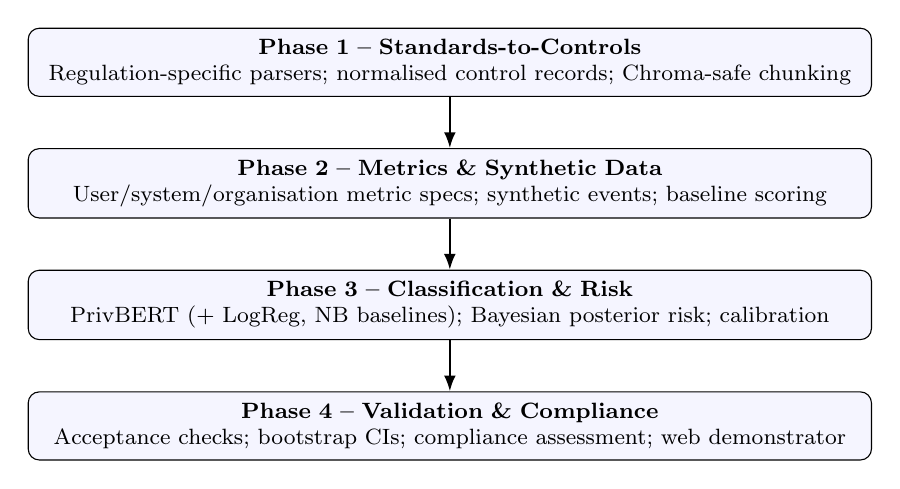
\begin{tikzpicture}[
  node distance=6.5mm,
  box/.style={draw, rounded corners, align=center, inner sep=4pt,
              text width=0.86\columnwidth, font=\footnotesize, fill=blue!4},
  data/.style={draw, align=center, inner sep=3pt,
               text width=0.86\columnwidth, font=\scriptsize\itshape, fill=gray!8},
  arr/.style={-{Latex[length=2mm]}, thick}]
\node[box] (p1) {\textbf{Phase 1 -- Standards-to-Controls}\\
  Regulation-specific parsers; normalised control records; Chroma-safe chunking};
\node[box, below=of p1] (p2) {\textbf{Phase 2 -- Metrics \& Synthetic Data}\\
  User/system/organisation metric specs; synthetic events; baseline scoring};
\node[box, below=of p2] (p3) {\textbf{Phase 3 -- Classification \& Risk}\\
  PrivBERT (+ LogReg, NB baselines); Bayesian posterior risk; calibration};
\node[box, below=of p3] (p4) {\textbf{Phase 4 -- Validation \& Compliance}\\
  Acceptance checks; bootstrap CIs; compliance assessment; web demonstrator};
\draw[arr] (p1) -- (p2);
\draw[arr] (p2) -- (p3);
\draw[arr] (p3) -- (p4);
\end{tikzpicture}
\caption{The four-phase PrERT-CNM-v4 pipeline. Each phase emits versioned
artefacts that are consumed as verified inputs by the subsequent phase.}
\label{fig:pipeline}
\end{figure}

A unifying abstraction is the three-level privacy taxonomy in
Table~\ref{tab:labelspace}, which maps OPP-115 data-practice categories onto
the \texttt{user}, \texttt{system}, and \texttt{organisation} levels. This
taxonomy is shared across phases: it defines the classifier label space, the
granularity of the metric specifications, and the structure of the Bayesian
posteriors.

\begin{table}[t]
\centering
\caption{Three-level privacy taxonomy used throughout the pipeline.}
\label{tab:labelspace}
\footnotesize
\begin{tabular}{@{}p{0.20\columnwidth} p{0.70\columnwidth}@{}}
\toprule
\textbf{Level} & \textbf{Representative OPP-115 categories} \\
\midrule
\texttt{user} & User Choice/Control; User Access, Edit \& Deletion \\
\texttt{system} & Data Security; Do Not Track \\
\texttt{organisation} & First-Party Collection/Use; Third-Party Sharing/Collection; Data Retention; Policy Change \\
\bottomrule
\end{tabular}
\end{table}

% =====================================================================
\subsection{Phase 1: Standards-to-Controls Extraction}\label{sec:phase1}
% =====================================================================
Phase~1 converts heterogeneous regulatory documents into a normalised,
machine-readable control catalogue. Rather than a single generic parser, the
system employs \emph{regulation-specific} parsers that respect each
document's structure: GDPR articles, ISO/IEC clauses and bullet hierarchies,
and NIST Privacy Framework subcategories are each handled by a dedicated
extractor. Each extracted control is stored as a record with a normalised
identifier (for example, \texttt{gdpr::Article\_32}), its hierarchical path,
the source text, and a parser-confidence score. Control text is then
segmented using a line-based chunking strategy to support downstream retrieval
and Chroma vector indexing~\cite{chroma_docs}. The resulting artefacts span GDPR,
ISO/IEC 27001/27002/27005/27018/27701/29100/29151, ISO/IEC
15944-12~\cite{iso15944_12_2020}, and the NIST Privacy Framework, and
provide the traceability backbone linking each clause to one or more
measurable indicators.

% =====================================================================
\subsection{Phase 2: Metrics, Synthetic Data, and Baseline Scoring}\label{sec:phase2}
% =====================================================================
Phase~2 translates Phase~1 controls into metric specifications, each defining
an identifier, scoring formula, required evidence fields, normalisation rule,
confidence weighting, and missing-data handling, at the user, system, and
organisation levels. To exercise the scoring logic under controlled
conditions, the pipeline generates synthetic observations across three
scenarios, \emph{normal}, \emph{stressed}, and \emph{adversarial}, with
deterministic seeding for reproducibility. Each observation records check
counts, failure counts, missing fields, and an observed-confidence value.
Baseline scoring then produces metric-level, level-summary, and
scenario-level results, establishing reference behaviour prior to the
introduction of learned components and providing a controlled substrate for
edge cases such as missing consent or delayed breach response. Public breach
attributes~\cite{enisa_tl_2024,prc_breaches} may optionally enrich these
observations.

% =====================================================================
\subsection{Phase 3: Clause Classification and Bayesian Risk}\label{sec:phase3}
% =====================================================================
Phase~3 is the analytical core. A clause classifier maps policy text to the
three-level taxonomy, and a Bayesian layer converts its probabilistic outputs
into standards-traceable risk posteriors. The implementation tracks five
artifact paths: the accepted release candidate (\texttt{phase-3-freeze}),
a same-split multinomial na\"ive-Bayes baseline (\texttt{phase-3}), and
three archived variant paths (\texttt{phase-3-privacybert},
\texttt{phase-3-logreg}, and \texttt{phase-3-no-bayes}) used for technique
coverage and ablation analysis.

\paragraph{Clause classification}
The primary classifier fine-tunes the PrivBERT privacy-policy checkpoint
\texttt{mukund/privbert}, introduced with the PrivaSeer corpus
\cite{srinath2021privaseer}, through Hugging Face Transformers
\cite{wolf2020transformers} and PyTorch~\cite{paszke2019pytorch}. To counter
the pronounced class imbalance of the corpus, training uses a class-weighted
focal-loss objective~\cite{lin2017focal}. Two ablation baselines are retained
for comparison: a sublinear TF-IDF logistic-regression model and a
multinomial na\"ive-Bayes classifier, both implemented with
scikit-learn~\cite{pedregosa2011scikit}.

\paragraph{Bayesian risk integration}
Classifier probabilities are aggregated into level-specific Beta--Bernoulli
posteriors. For each level $\ell \in \{\text{user}, \text{system},
\text{organisation}\}$, a prior $\mathrm{Beta}(\alpha_0, \beta_0)$ encoding
standards expectations is updated with observed clause-level evidence to
yield a posterior $\mathrm{Beta}(\alpha_\ell, \beta_\ell)$, whose mean
provides the level risk score and whose $2.5$th and $97.5$th percentiles
furnish a 95\% credible interval following standard Bayesian updating
\cite{gelman2013bayesian}. Each posterior retains its top-contributing
clauses, preserving an auditable trace from the aggregate score back to
individual policy statements and, through Phase~1, to the originating
standard.

% =====================================================================
\subsection{Phase 4: Validation, Calibration, and Compliance}\label{sec:phase4}
% =====================================================================
Phase~4 validates the Phase~3 artefacts against explicit acceptance criteria.
Blocking checks confirm the presence of the expected artefacts, the absence
of policy-level train/validation/test leakage, the satisfaction of core
metric thresholds, and the schema validity and count consistency of the
prediction records. Calibration is quantified by the expected calibration
error (ECE)~\cite{guo2017calibration} and the Brier
score~\cite{brier1950verification}, and statistical uncertainty is
characterised by stratified bootstrap confidence
intervals~\cite{efron1993bootstrap}. A separate compliance-assessment module
scores arbitrary policy text against weighted checks, covering consent and
transparency, user rights, data security, data minimisation, retention,
third-party sharing, and personally identifiable information protection.
The latest revision adds a policy-only mode that emits independent
per-regulation verdicts (GDPR, NIST Privacy Framework, ISO/IEC 27701)
with explicit supporting clause citations, enabling transparent
cross-framework reasoning without a required schema input. A Gradio web
demonstrator exposes the full pipeline interactively for local or temporary
public review~\cite{gradio_docs,huggingface_spaces_docs}.

% =====================================================================
\section{Experimental Setup}\label{sec:setup}
% =====================================================================
\subsection{Datasets}
The canonical training and evaluation corpus is OPP-115~\cite{wilson2016opp115,opp115_dataset},
consolidated at a 0.75 inter-annotator agreement threshold and mapped onto
the three-level taxonomy. The July~2026 freeze uses OPP-115 as the sole
training and evaluation anchor; auxiliary APP-350 ingestion is implemented
but disabled in the accepted freeze because the conservative mapping did not
provide balanced coverage of the project label space. Polisis-derived
data~\cite{harkous2018polisis} are supported for category harmonisation, and
public breach corpora~\cite{enisa_tl_2024,prc_breaches} inform Phase~2 enrichment.

\subsection{Data Partitioning and Leakage Control}
To prevent optimistic bias from near-duplicate clauses, the corpus is split
\emph{by policy}: all clauses from a given policy reside in exactly one
partition. The accepted freeze splits comprise $15{,}484$ training rows (92
policies), $1{,}764$ validation rows (11 policies), and $2{,}472$ test rows
(12 policies), from $19{,}720$ total rows. Verified pairwise policy overlap between every pair of
partitions is zero. The corpus is markedly imbalanced, approximately 84\%
\texttt{organisation}, 12\% \texttt{user}, and 4\% \texttt{system}, which
directly motivates the focal-loss objective and the use of macro-averaged
metrics. Archived variant runs retained for technique coverage were produced
on an earlier split family (1803 validation / 2272 test) and are reported
with explicit non-comparability caveats in Section~\ref{sec:results}.

\subsection{Model Configuration}
The freeze classifier fine-tunes \texttt{mukund/privbert} for two epochs with
a batch size of 8, a learning rate of $5\times10^{-5}$, a maximum sequence
length of 256 tokens, weight decay of $0.01$, focal loss ($\gamma = 2.0$),
and early stopping with patience 1. A fixed random seed of 42 governs all
stochastic operations. Calibration uses 10 reliability bins and uncertainty
estimates use 1{,}000 bootstrap resamples.

\subsection{Evaluation Metrics}
Classification quality is reported as accuracy and macro-averaged precision,
recall, and F1, the latter chosen to weight minority classes equally under
imbalance. Calibration is reported as ECE and the Brier score, and all
headline metrics are accompanied by 95\% bootstrap confidence intervals. The
Bayesian layer is summarised by its primary posterior score and per-level
credible intervals.

% =====================================================================
\section{Results}\label{sec:results}
% =====================================================================
\subsection{Model Comparison}
Table~\ref{tab:modelcomp} reports the accepted freeze model together with all
tracked Phase~3 variants. The July~2026 PrivBERT freeze (accepted) achieves a
test macro-F1 of $0.869$ and accuracy of $0.954$, improving on the same-split
na\"ive-Bayes baseline by $21.9$ macro-F1 points and $13.3$ accuracy points.
Archived variant rows are included for technique coverage and ablation
completeness, but were generated on an earlier policy split and are therefore
not interpreted as same-split acceptance comparisons.

\begin{table}[t]
\centering
\caption{Phase~3 classifier comparison on OPP-115 (macro-F1 and accuracy).}
\label{tab:modelcomp}
\scriptsize
\setlength{\tabcolsep}{3pt}
\begin{tabular}{@{}l cccc@{}}
\toprule
& \multicolumn{2}{c}{\textbf{Validation}} & \multicolumn{2}{c}{\textbf{Test}} \\
\cmidrule(lr){2-3}\cmidrule(lr){4-5}
\textbf{Model} & Macro-F1 & Acc. & Macro-F1 & Acc. \\
\midrule
\textbf{PrivBERT freeze (S1)} & \textbf{0.935} & \textbf{0.973} & \textbf{0.869} & \textbf{0.954} \\
Na\"ive Bayes baseline (S1) & 0.704 & 0.842 & 0.649 & 0.821 \\
PrivacyBERT variant (S0) & 0.872 & 0.951 & 0.892 & 0.956 \\
LogReg TF-IDF variant (S0) & 0.758 & 0.890 & 0.779 & 0.893 \\
LogReg TF-IDF no Bayes (S0) & 0.758 & 0.890 & 0.779 & 0.893 \\
\bottomrule
\end{tabular}
\\[-0.5ex]
{\scriptsize S1: accepted split (1764/2472). S0: archived split (1803/2272).}
\end{table}

\subsection{Per-Class Performance}
Table~\ref{tab:perclass} details the freeze classifier's per-class behaviour
on the test set. The majority \texttt{organisation} class remains strongest
(F1 $0.973$), while the minority \texttt{user} class reaches F1 $0.879$ and
the smaller \texttt{system} class reaches F1 $0.754$. This residual gap is
the principal target for future data augmentation and prior-sensitivity work.

\begin{table}[t]
\centering
\caption{Per-class test metrics for the PrivBERT freeze classifier.}
\label{tab:perclass}
\footnotesize
\begin{tabular}{@{}l cccc@{}}
\toprule
\textbf{Class} & \textbf{Precision} & \textbf{Recall} & \textbf{F1} & \textbf{Support} \\
\midrule
\texttt{user}         & 0.884 & 0.874 & 0.879 & 278 \\
\texttt{system}       & 0.735 & 0.773 & 0.754 & 97 \\
\texttt{organisation} & 0.974 & 0.973 & 0.973 & 2{,}097 \\
\midrule
\textbf{Macro avg.}   & 0.864 & 0.873 & 0.869 & 2{,}472 \\
\bottomrule
\end{tabular}
\end{table}

\subsection{Calibration and Uncertainty}
The freeze classifier is well calibrated, with a test ECE of $0.0525$ and a
Brier score of $0.0400$ over ten reliability bins; the macro-averaged
one-vs-rest ECE is $0.0460$.
Stratified bootstrap resampling ($n = 1{,}000$) yields a 95\% confidence
interval of $[0.845, 0.892]$ for test macro-F1 and $[0.946, 0.962]$ for test
accuracy, confirming that the headline results are statistically stable
rather than artefacts of a single favourable split. Because calibration and
bootstrap outputs are acceptance-gating criteria in the freeze path, they are
reported for the accepted split and not used to rank archived
non-comparable variants.

\subsection{Bayesian Risk Posteriors}
The Bayesian layer produces a primary posterior score of $0.901$ on the test
set. Level-specific posteriors retain the imbalance signal: \texttt{user}
mean $0.837$ with 95\% interval $[0.794, 0.880]$ from 275 evidence records,
\texttt{system} mean $0.863$ with interval $[0.798, 0.928]$ from 102 records,
and \texttt{organisation} mean $0.911$ with interval $[0.899, 0.923]$ from
2{,}095 records. Each posterior is accompanied by its highest-confidence
contributing clauses, preserving traceability from the aggregate score to
individual policy statements.

\subsection{Auxiliary Corpus Gatekeeping}
APP-350 preprocessing is implemented as a controlled, training-only auxiliary
path, but the accepted freeze disables auxiliary rows. The conservative
mapping did not provide balanced coverage of the \texttt{user}, \texttt{system},
and \texttt{organisation} labels, so the canonical results remain anchored to
OPP-115 only. This design choice keeps the held-out evaluation interpretable
and avoids presenting auxiliary data as beneficial before a defensible label
mapping is available.

\subsection{Phase 4 Compliance Output Update}
Beyond acceptance validation, the updated Phase~4 assessor supports a
policy-only compliance path that emits check-level outcomes and
framework-specific verdict objects with clause citations. This extends the
earlier aggregate compliance score into a traceable evidence view across GDPR,
NIST Privacy Framework, and ISO/IEC 27701 controls. Current repository outputs
include demonstrator reports generated on synthetic policy snippets; these are
treated as workflow evidence rather than as a benchmark of real-world policy
compliance prevalence.

% =====================================================================
\section{Discussion}\label{sec:discussion}
% =====================================================================
The results substantiate the central claim that clause-level NLP and
standards-traceable probabilistic scoring can be productively unified. Four
observations stand out. First, calibration matters as much as accuracy: a
classifier feeding a downstream risk model must report trustworthy
probabilities, and the observed ECE of $0.0525$ indicates that the freeze
classifier's confidence can be propagated into the Bayesian layer without
aggressive re-calibration. Second, class imbalance is the dominant obstacle to further
gains; the minority \texttt{system} class, with only 97 test instances,
caps macro-F1 despite strong majority-class performance, and focal loss
mitigates but does not eliminate this effect. Third, split discipline is
critical for interpretation: archived variants may show higher point
estimates than the accepted freeze, but on different partition sizes and are
therefore unsuitable for direct acceptance comparison. Fourth, traceability is a
first-class design property rather than an afterthought: because every
posterior retains its contributing clauses and every clause is linked through
Phase~1 to a specific standard, the framework can answer not only ``how risky''
but ``why, and against which obligation'', a capability absent from prior
clause-classification systems~\cite{harkous2018polisis,muralitharan2024privacybertlstm}.

% =====================================================================
\section{Limitations and Threats to Validity}\label{sec:limitations}
% =====================================================================
Several limitations temper these findings. \emph{Construct validity}: the
three-level taxonomy is a deliberate simplification of the ten-category
OPP-115 scheme, which eases risk aggregation but discards fine-grained
distinctions. \emph{External validity}: evaluation centres on OPP-115;
although policy-level splitting controls within-corpus leakage, generalisation
to policies drafted under different legal regimes or in other languages is
untested, and the APP-350 gatekeeping result shows that na\"ive corpus
augmentation can harm label coverage before it helps model quality.
\emph{Internal validity}: the Bayesian priors encode
analyst judgement about standards expectations, and the high primary posterior
score partly reflects these prior choices; sensitivity analysis over priors is
left to future work. Finally, synthetic Phase~2 data are used to exercise
scoring logic rather than to make empirical claims, and should not be read as
evidence of real-world risk levels.

% =====================================================================
\section{Ethical and Data-Governance Considerations}\label{sec:ethics}
% =====================================================================
The project involves no human participants and collects no personal data. All
training and evaluation data are pre-existing public research corpora or
synthetically generated records, placing the work in the lowest-risk ethics
tier under Kingston University's self-certification process. Synthetic events
contain no identifiable information, and the public breach
datasets~\cite{enisa_tl_2024,prc_breaches} comprise incident summaries rather
than personal records. Use of OPP-115 complies with its research-and-teaching
licence. Ethical deployment constraints remain central: (i) model outputs are
probabilistic and may under-represent minority disclosure patterns;
(ii) compliance verdicts are evidence-linked but not legal determinations;
and (iii) per-regulation scoring should be reviewed by domain experts before
operational decisions are made. The framework is intended as a
decision-support and transparency aid; its scores are advisory and should not
substitute for qualified legal assessment of compliance.

% =====================================================================
\section{Conclusion and Future Work}\label{sec:conclusion}
% =====================================================================
This paper introduced PrERT-CNM-v4, an AI-driven, standards-aligned framework
for quantifying user privacy risk. By coupling a calibrated PrivBERT-backed
clause classifier (test macro-F1 $0.869$; ECE $0.0525$) with a
standards-traceable Bayesian risk layer, the framework bridges the long-standing gap between
automated policy analysis and regulatory measurement, while a reproducible
four-phase pipeline with explicit acceptance criteria underpins its
trustworthiness. The updated implementation further contributes a
variant-tracked Phase~3 evaluation stack and a policy-only Phase~4
cross-regulation compliance pathway with auditable clause citations.
Future work will pursue three directions: domain-adaptive
pre-training and targeted augmentation to lift minority-class performance;
sensitivity analysis and elicitation procedures for the Bayesian priors; and
external validation against multilingual and cross-jurisdictional policy
corpora, together with empirical anchoring of risk scores to observed breach
outcomes.

% =====================================================================
\section*{Acknowledgements}
% =====================================================================
The author thanks Dr Razi Arshad for supervisory guidance throughout this MSc
research project at Kingston University.

% =====================================================================
% REFERENCES
% =====================================================================
\bibliographystyle{IEEEtran}
\bibliography{references}

\end{document}
